\documentclass[main]{subfiles}
\begin{document}

%%@@@@@@@@@@@@@@@@@@@@@@@@@@@@@@
%\noindent
%\textbf{Topics: Feed-Forward Networks and Backpropagation - 03.12.2020} \\
%Lecturer: Dr. Matthew Cook \\
%Author: Vanessa Leite \{vanessa at ini.uzh.ch\}

\section{Feed-Forward Networks}

Feed-forward networks (FFN) are not like the networks in the brain.
In the feed-forward networks, the information moves in only one direction (forward) from the input nodes, through the hidden nodes (if they exist), and to the output nodes.
\textbf{There are no cycles in this network.}
Usually, people are referring to feed-forward networks when they talk about artificial neural networks (ANN).

General structure:
\begin{itemize}[noitemsep,nolistsep]
	\item Multiple layers of neurons with a certain number of inputs and outputs.
	\item Every layer of nodes feeds the next layer with inputs.
	\item Each input in one layer is connected to all the inputs in the next layer.
	\item There is an input and an output layer with hidden layers in between.
\end{itemize}

\begin{figure}[H]
	\centering
	\includegraphics[width=0.3\textwidth]{Feed_forward_neural_net.png}
	\caption{Example of a feed-forward network with an input layer, a hidden layer and an output layer.}
\end{figure}

A single unit, like a perceptron, can be seen as a feed-forward network.

We can write down the connections of a FFN as a matrix of weights, so $w_{ij}$ is the weight from $i$ to $j$.

Why FFN are nice?
Because we can think about functions that receive inputs and generate outputs.
When we use FFN we know what we want to compute.
We need to set the weights of the network in oreder to compute the function we want.
The process of defining the weights is called learning or training.

In feed-forward networks it is easy to evaluate each unit.
The outputs are continuous functions of the input, which facilitates the optimization in case of wrong outputs.
The training can be done using "training data": input/output pairs ($x_i, d_i)$. Where $x_i$ is the input value and $d_i$ is the desired output.
Then we can define the error $E = \Sigma_k (f(x_k) - d_k)^2$, where $f(x_k)$ is the output of the network.
Differently of hopfield networks, we don't need continuous updates and we do not reevaluate units.
FFN have the idea of a pipeline (not like the brain).

If a node on layer $n$ in a FFN is connected to layer $n+i$ with $i > 1$, this is still a FFN, however the most common structure is to connect nodes on layer $n$ to nodes on layer $n+1$.


How can we change the weights to reduce the error?
We can use gradient descent.
We calculate all the $\frac{\partial E}{\partial w_i}$ in the network, easily, by starting at the end and then walking backwards. This is known as Backpropagation.

\textbf{Training process}
\begin{enumerate}
\item Give to the network an input.
\item Calculate all the values in the network to produce the output.
\item Compare output with the desired output.
This gives us the "error" for this input.
\item Update the weights.
For example, use gradient descent to optimize the parameters to minimize the error.
\end{enumerate}


\subsection{Backpropagation and Error function}
Backpropagation is the process of calculating the derivatives, using the chain rule, from the last layer (directly connected with the output, thus, with the loss function) to the first layer (connected with the inputs).
This process can be seen as walking through the network in a backwards manner.

\begin{itemize}[noitemsep,nolistsep]
	\item The inputs and desired outputs are given as $S=\{(x,d)^1,\ldots,(x,d)^l\}$.
	\item The error function is given as $E(S) = \sum_i\frac{1}{2}||y(x^i)-d^i||^2$.
	\item The output is a non-linear transformation $y=f(a)$.
	\item $f(a)$ is the activation function, which is usually a sigmoid function.
	\item The error function for a single training sample is $E(S)=\frac{1}{2}(f(x_1w_1+x_2w_2+w_0)-d)^2$.
	\item The output of a simple network is for example $y(x_1,x_2,x_3)=f(x_1w_{21}+f(x_2w_{11}+x_3w_{12}+w_{10})w_{22}+w_{20})$.
	\item $\frac{\partial E(w_1,w_2,w_0)}{\partial w_1}=(f(x_1w_1+x_2w_2+w_0)-d)\cdot f'(x_1w_1+x_2w_2+w_0)\cdot x_1$.
	\item $\frac{\partial E(w_1,w_2,w_0)}{\partial w_2}=(f(x_1w_1+x_2w_2+w_0)-d)\cdot f'(x_1w_1+x_2w_2+w_0)\cdot x_2$.
	\item $\frac{\partial E(w_1,w_2,w_0)}{\partial w_0}=(f(x_1w_1+x_2w_2+w_0)-d)\cdot f'(x_1w_1+x_2w_2+w_0)$.
	\item The error terms travel backwards through the network and get multiplied with the derivative of the activation function of that input. Multiple error terms can just be added up.
	\item The partial derivative of the error $E$ term in relation to the weight $w$ to be adjusted can be added to the weight in order to learn. An additional weighting factor can be added.
\end{itemize}

\subsection{Gradient Descent}
Consider $E = \sum(f_w(x) - y_i)^2$, we want to adjust $\vec{w}$ (weights of the network) to minimize $E$.
Gradient descent is the process of descending through the gradients (using the derivatives calculated with backpropagation), in this algorithm we try to reach the minimum of the loss function.
This is an iterative process.

Generally, the iterative process is given by $\theta_{i_{new}} = \theta_i + \Delta \theta_i$, where $\Delta \theta_i = - \alpha \frac{\partial J(\theta)}{\partial \theta_i}$.

\begin{figure}[H]
	\centering
	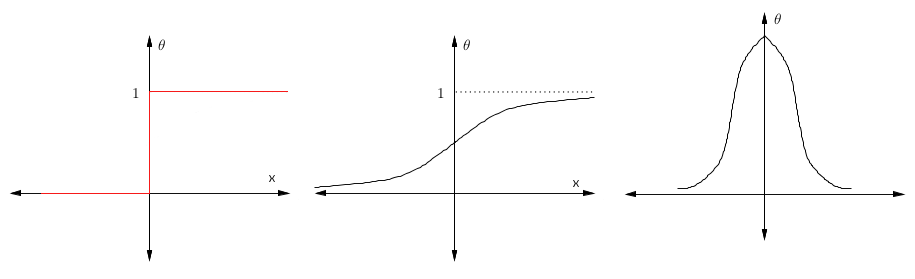
\includegraphics[width=0.6\textwidth]{activation-functions.png}
	\caption{left-most figure: $f_{w_0} (x) = \theta(wf + w...)$, $\frac{df}{dw} = 0 \rightarrow \theta$ is not a good threshold function.
To know in what direction we should move to find our minima, we need to use a threshold function that is continuous and differentiable, like the one in the center figure.
Right figure: $\frac{df}{dw} = \theta\prime$.}
\end{figure}

We haven't found biological mechanism that would be similat to gradient descent in the brain.


\subsection{Boltzmann Machines}

Boltzmann Machines were invented in 1985 but not by Boltzmann.
The name is given because these units use a Boltzmann distribution in their sampling function.

These units are similar to Hopfield Networks, however, they have a probability of being active.
When updating a unit, we set its value to zero or one probabilistically, following a sampling function, see Figure~\ref{fig:step-sigmoid-function}.
Boltzmann machines do not converge, they do not reach a stable state.
It can be seen as a system for sampling. It's a way to do a random walking in the state space.

\paragraph{Sampling}
There are many types of distributions.
When we want to get examples of these distributions, we need to sample from it.
And giving some samples we can recovery the distribution of the data.

\begin{figure}[H]
	\centering
	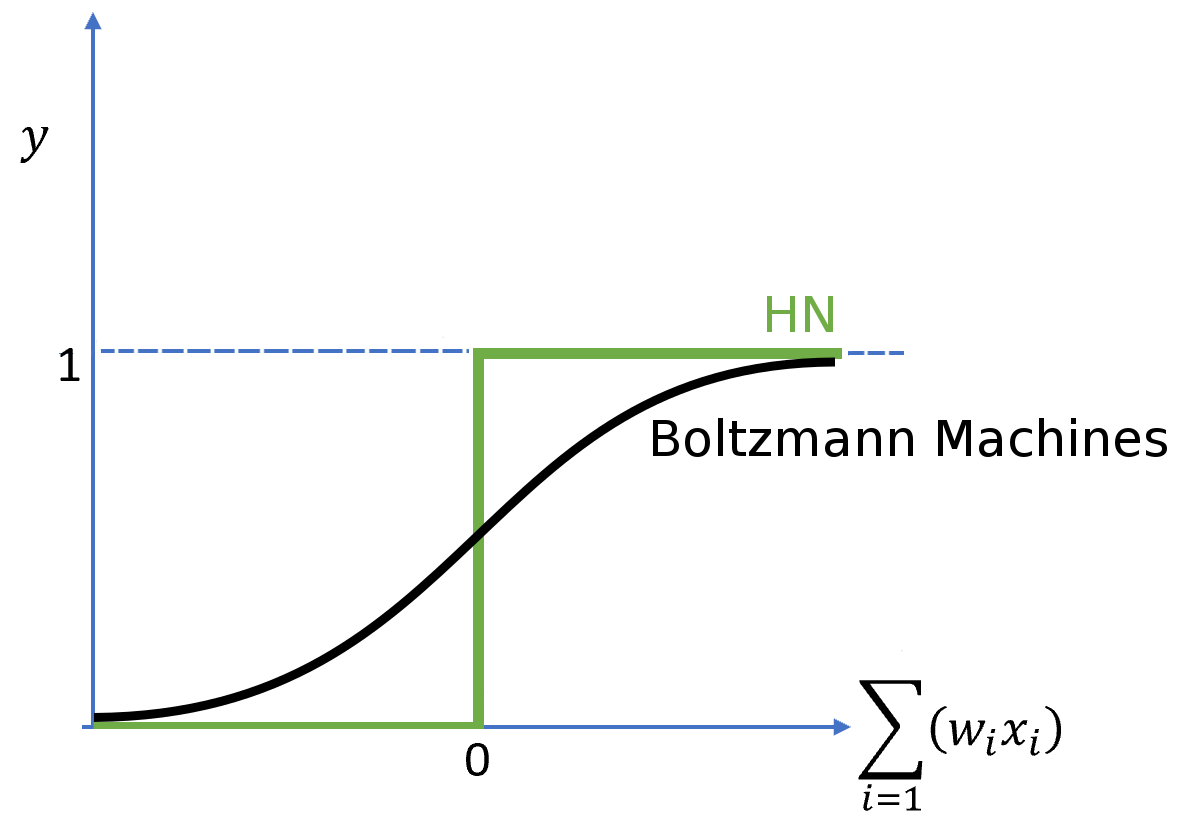
\includegraphics[width=0.5\textwidth]{step-sigmoid-function.png}
	\caption{Representations of activation function for Hopfield Networks (HN) and Boltzmann Machines}
	\label{fig:step-sigmoid-function}
\end{figure}

We want the units to forget previous states so the sampling is not biased, i.e., not similar to previous ones, thus really "random".
While this sampling is nice, it is not useful as a memory, i.e., we don't want to sample things randomly from our memory.

We can define a network where the units have a real-valued activity level ($a_i \in [0,1]$), and also we can make time continuous, so $\frac{\partial a_i}{\partial t} = \theta(\Sigma)-a_i$.

Using units like this, we can make a feed-forward network.


\end{document}
